\begin{frame}
\frametitle{Ringmap Packet Capturing Stack}
\begin{itemize}
	\item \textbf{Ringmap}: The new packet capturing stack
	\item based on standard FreeBSD packet capturing stack: 		
		\begin{itemize}
			\item based on generic network drivers and \emph{libpcap}
			\begin{itemize}
				\item but network driver and \emph{libpcap} require small
					modifications\newline
			\end{itemize}
		\end{itemize}
\end{itemize}
\end{frame}

\begin{frame}
	\frametitle{What did we change in \emph{generic}}
\begin{columns}
\column[t]{0.5\textwidth}
\begin{itemize}
	\item <2->Disabled TCP/IP-Stack
		\begin{itemize}
			\item Only packet capturing\newline
		\end{itemize}
	\item <3->BPF is accessible in both kernel and user-space\newline
	\item <4->Network driver and Libpcap is modified
		\begin{itemize}
			\item BPF is unchanged
		\end{itemize}
\end{itemize}
\column[t]{0.5\textwidth}
\vspace{-2em}
\only<1>{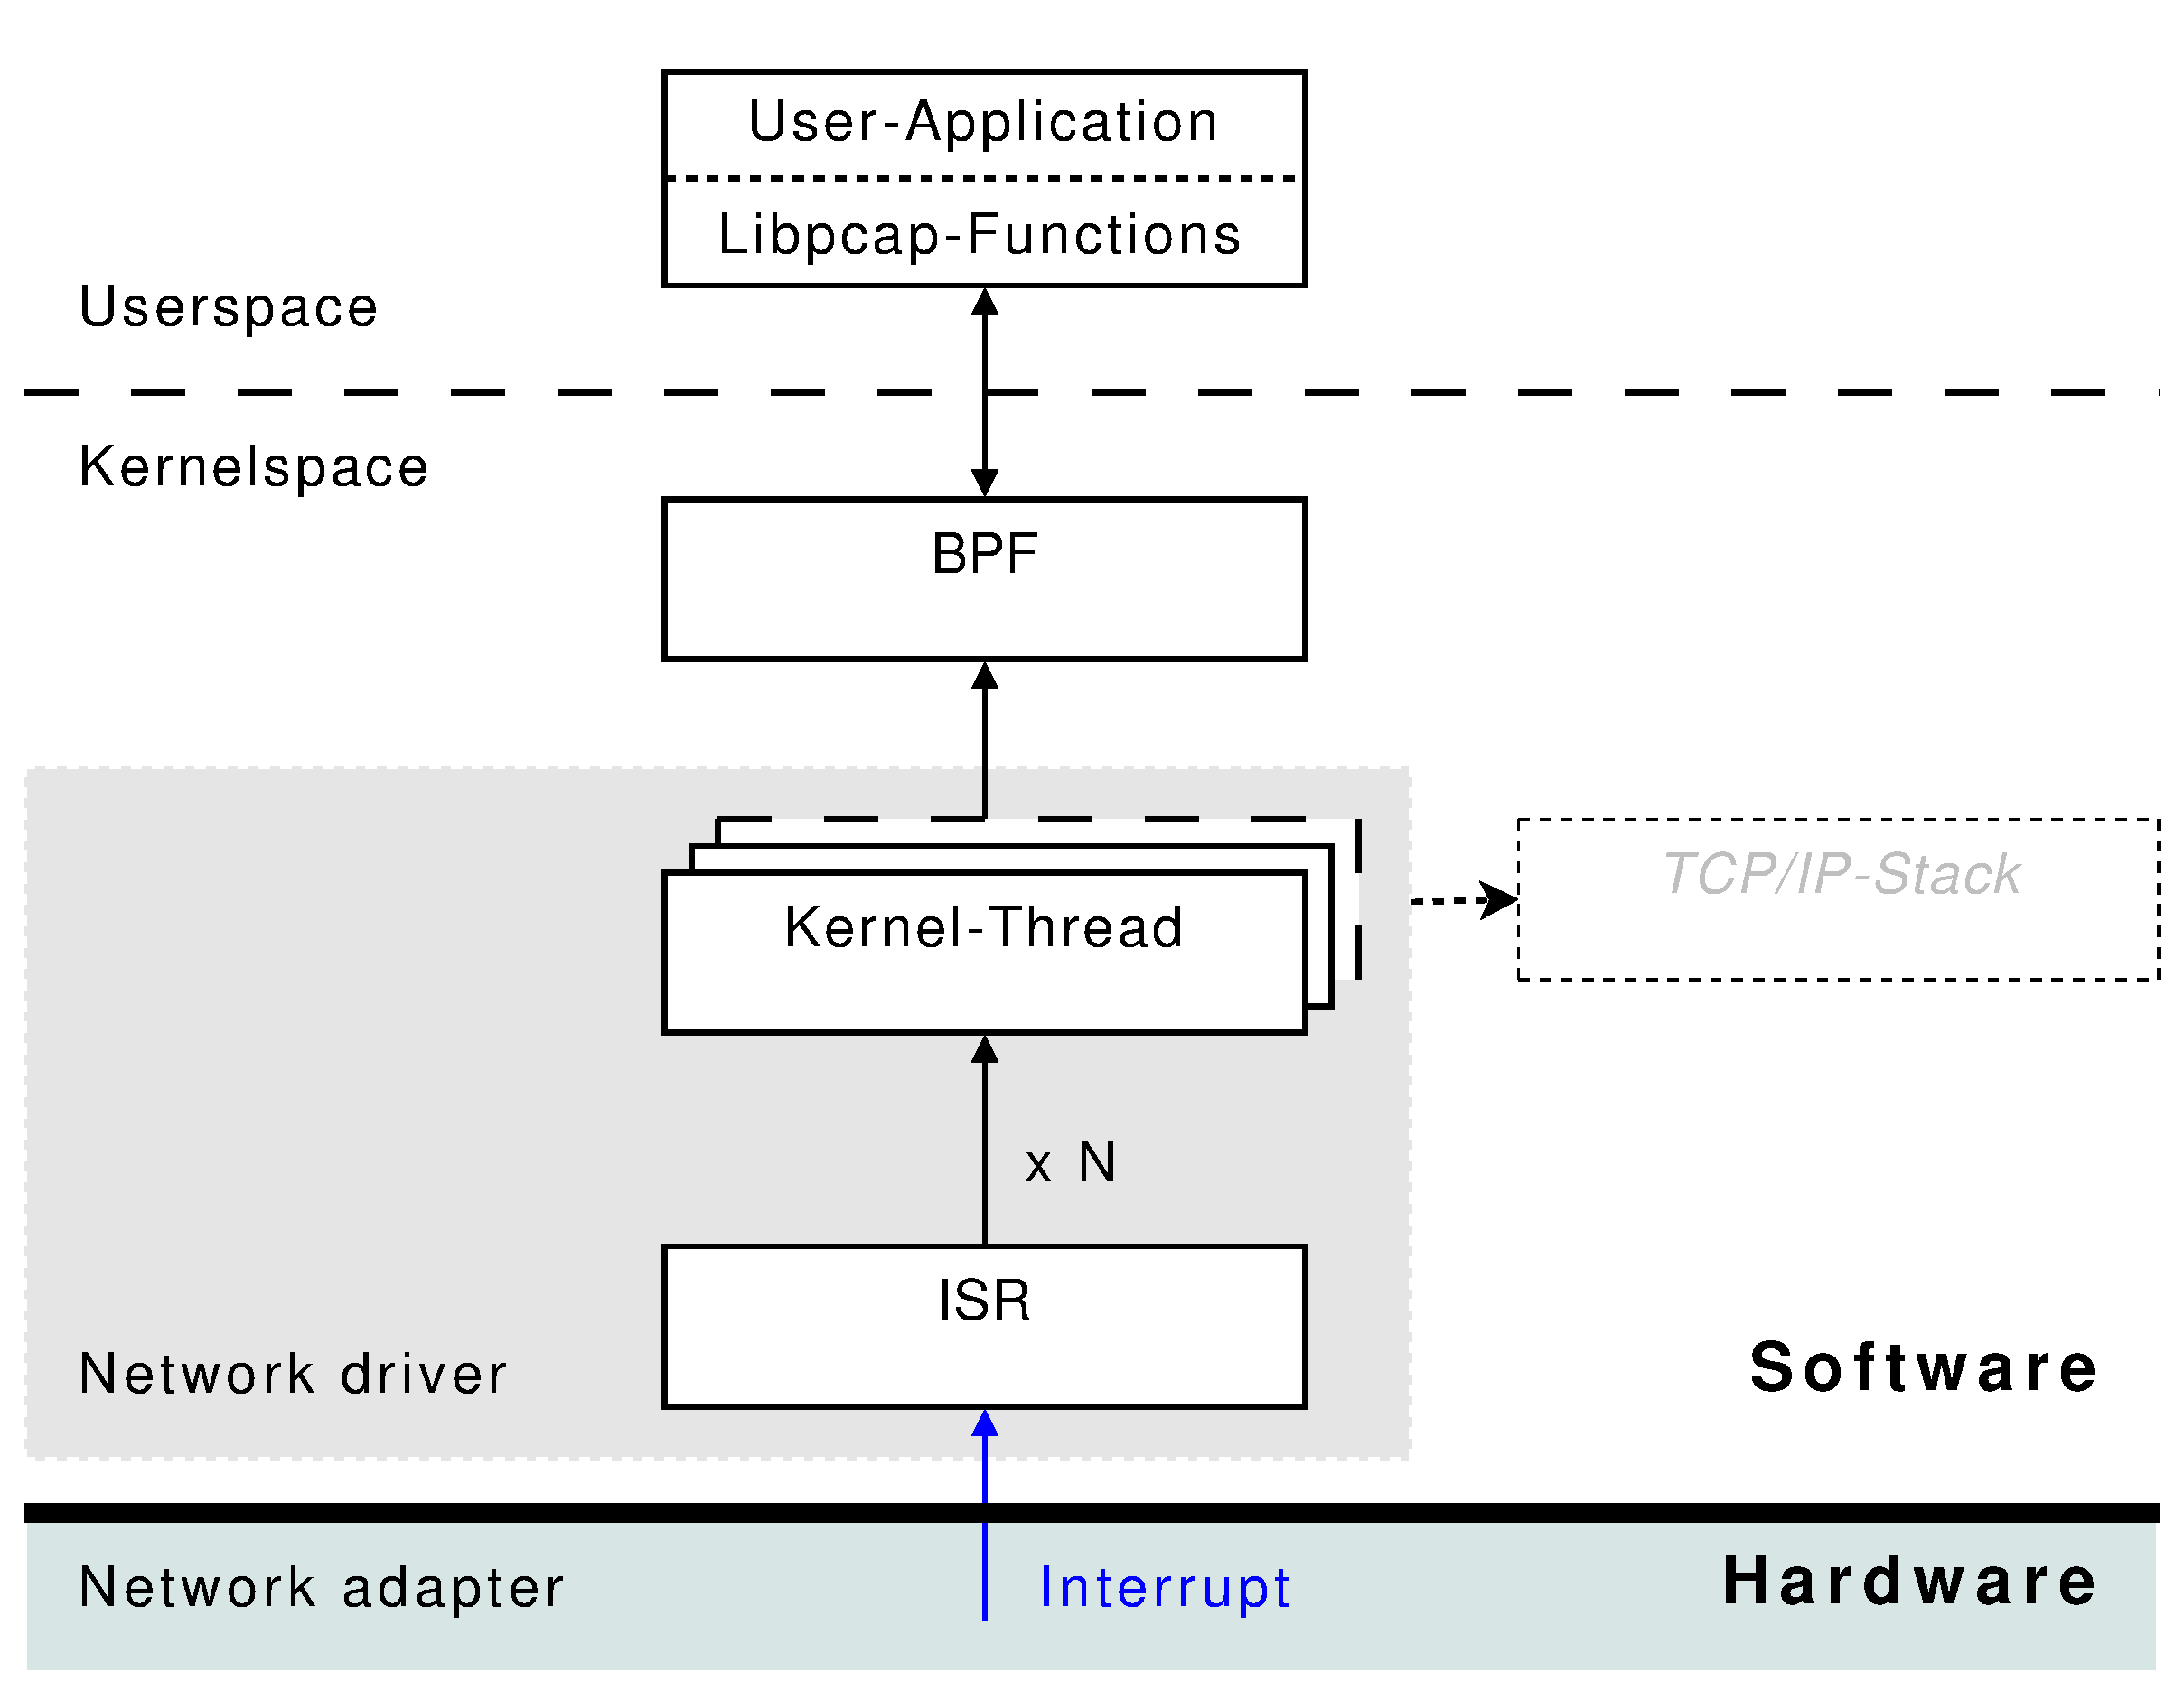
\includegraphics [height=55mm,width=60mm]{pics/PCS_funcs_ziel_DA_0}}
\only<2>{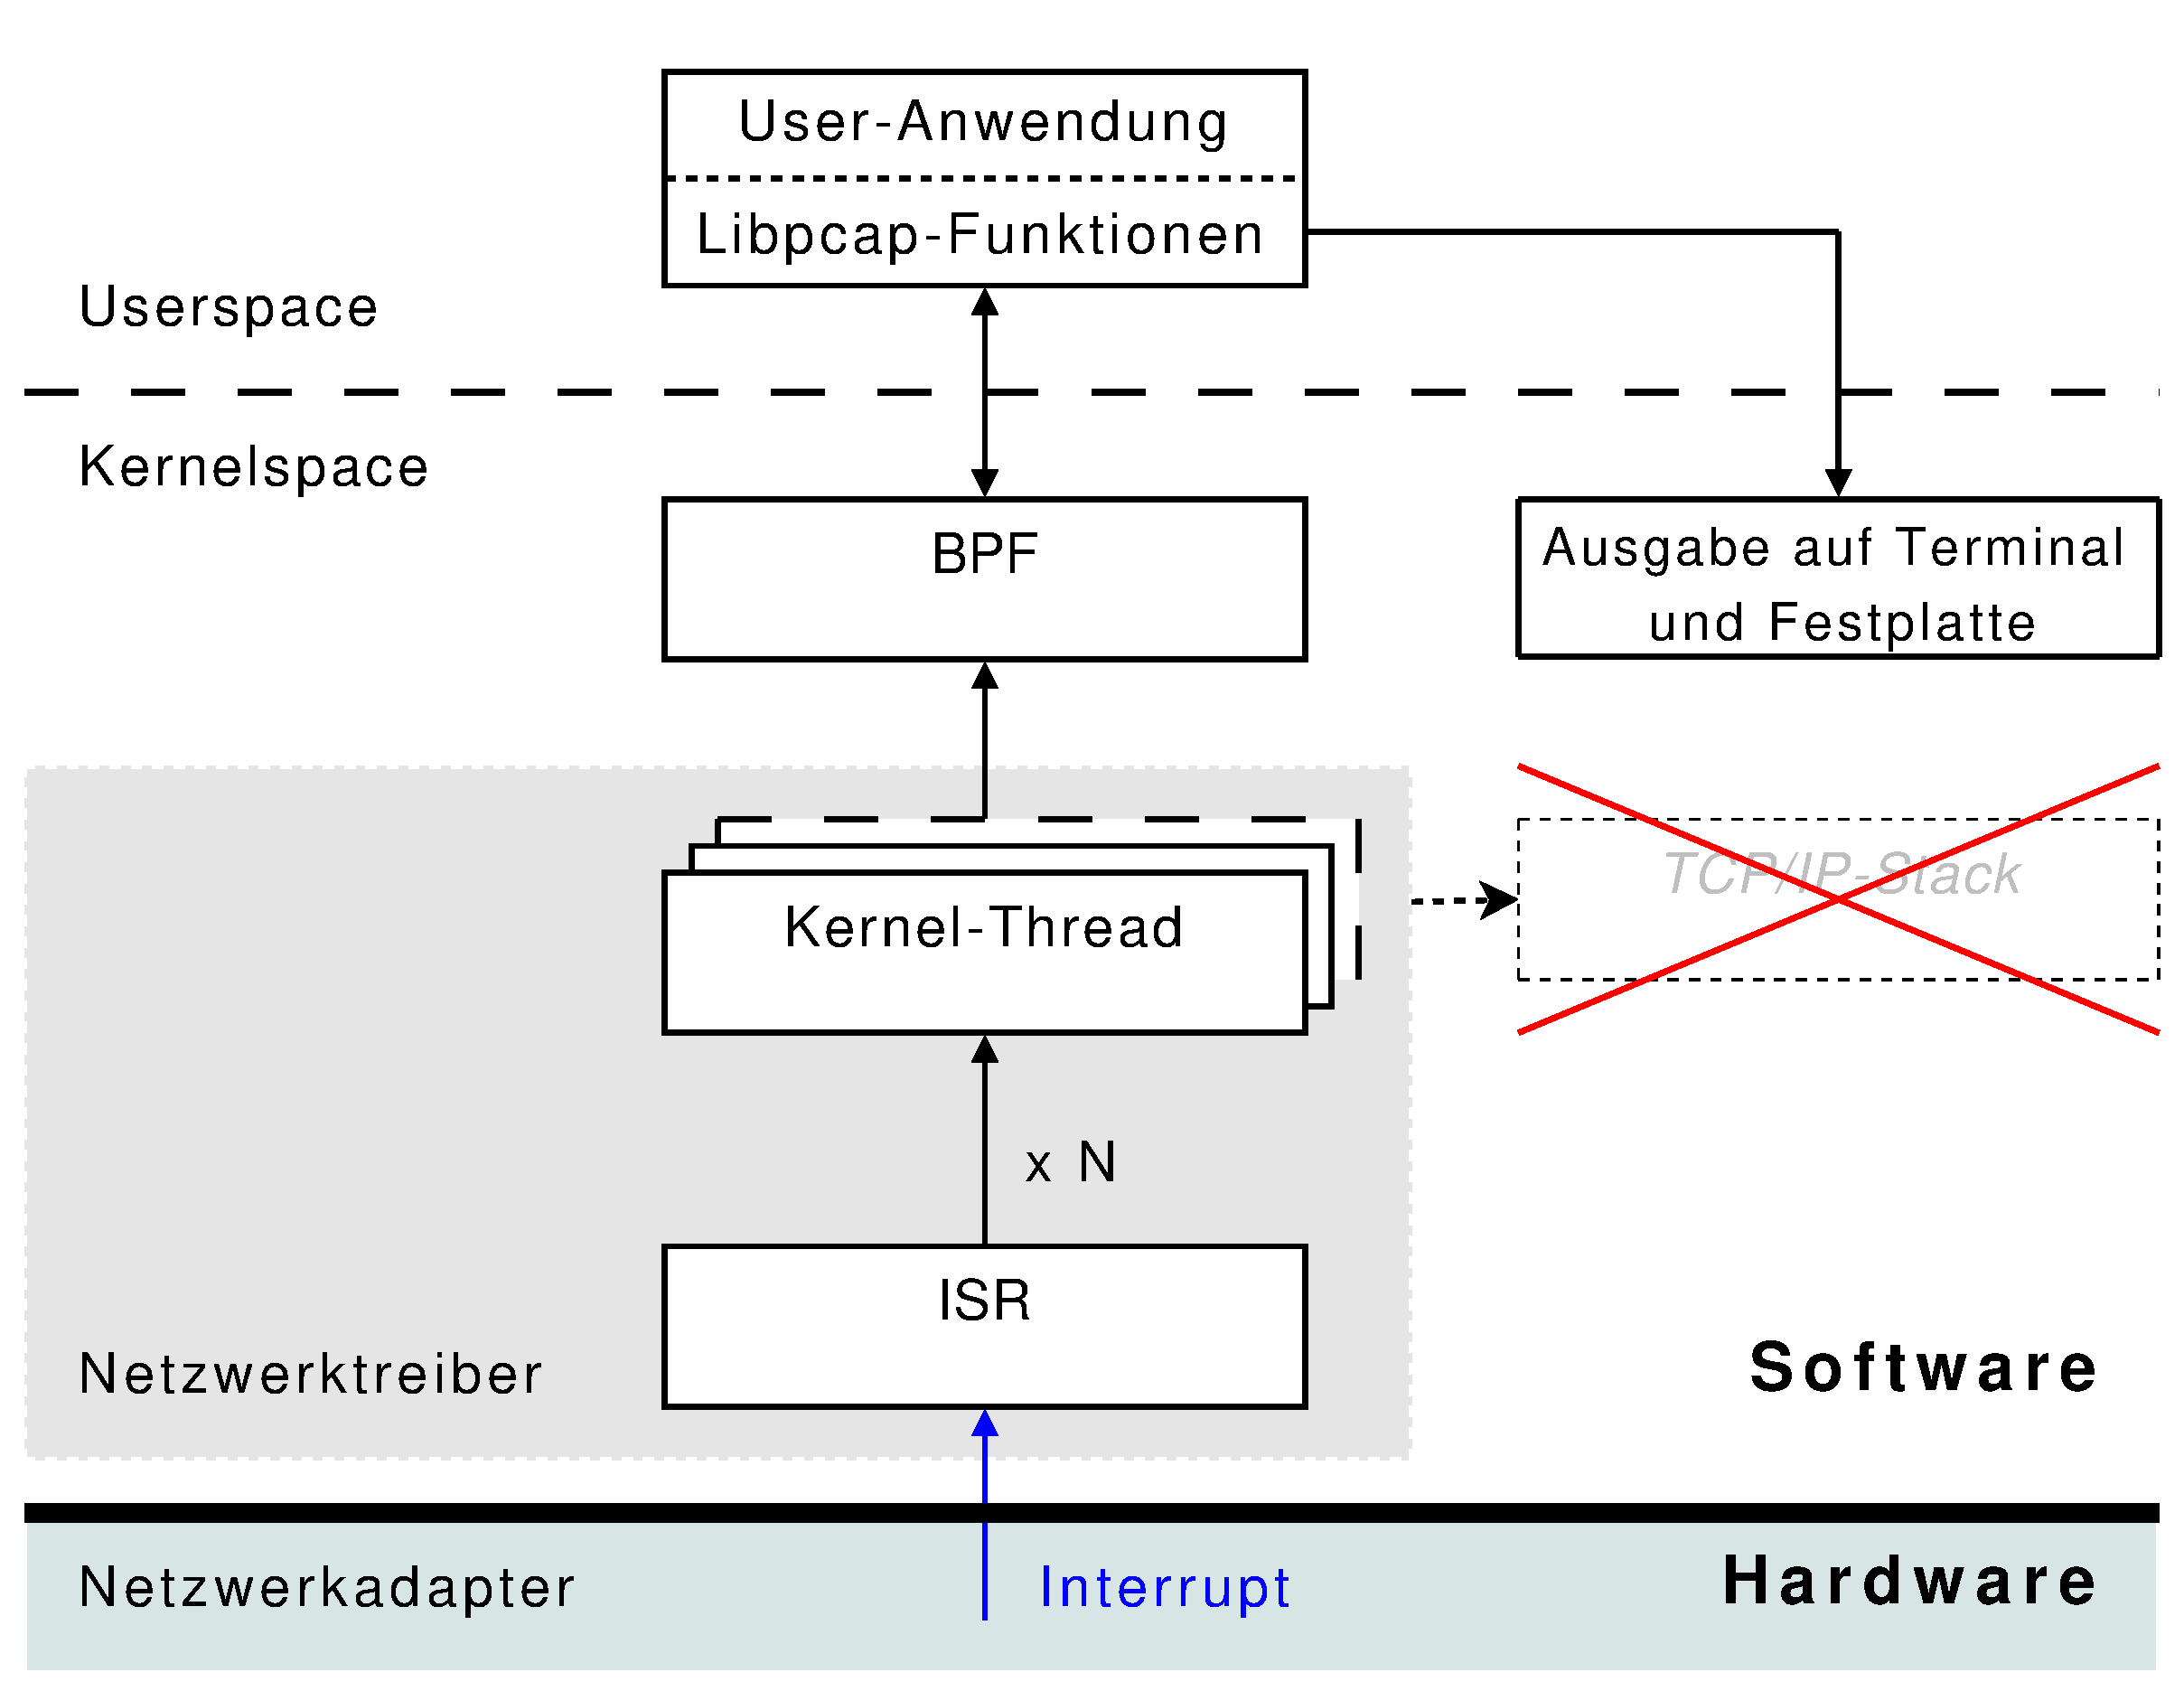
\includegraphics [height=55mm,width=60mm]{pics/PCS_funcs_ziel_DA_1}}
\only<3>{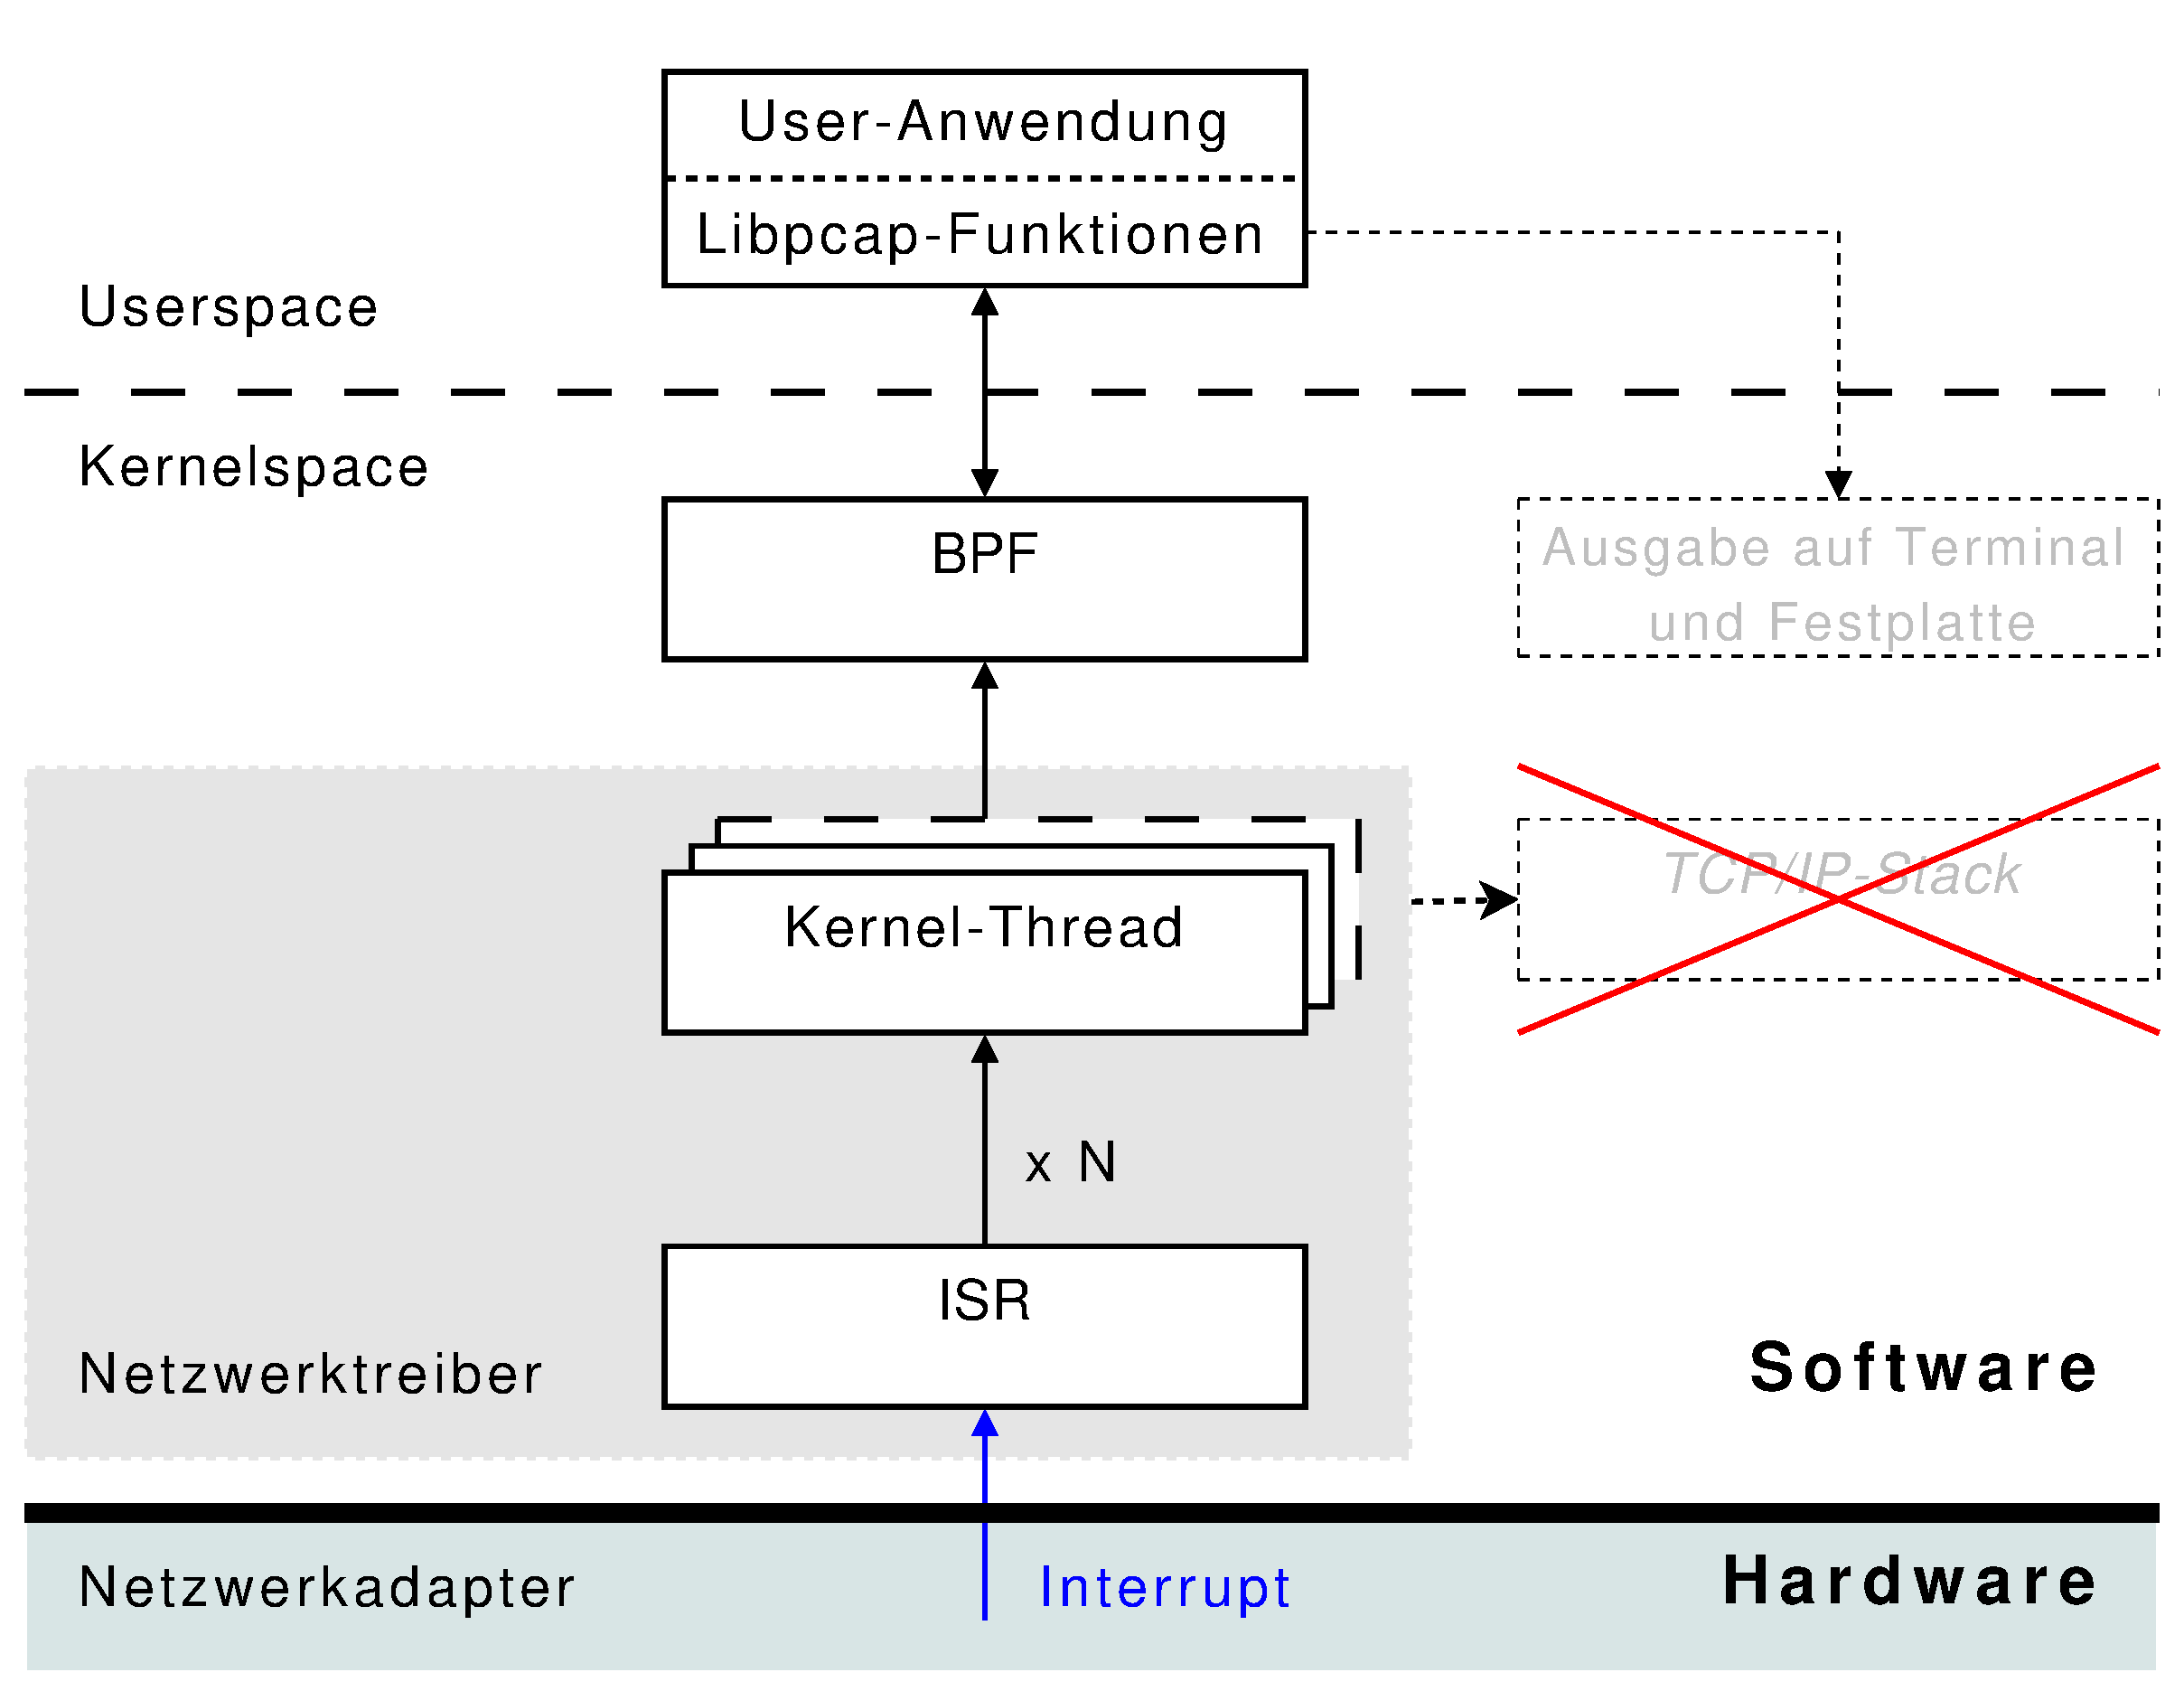
\includegraphics [height=55mm,width=60mm]{pics/PCS_funcs_ziel_DA_2}}
\only<4>{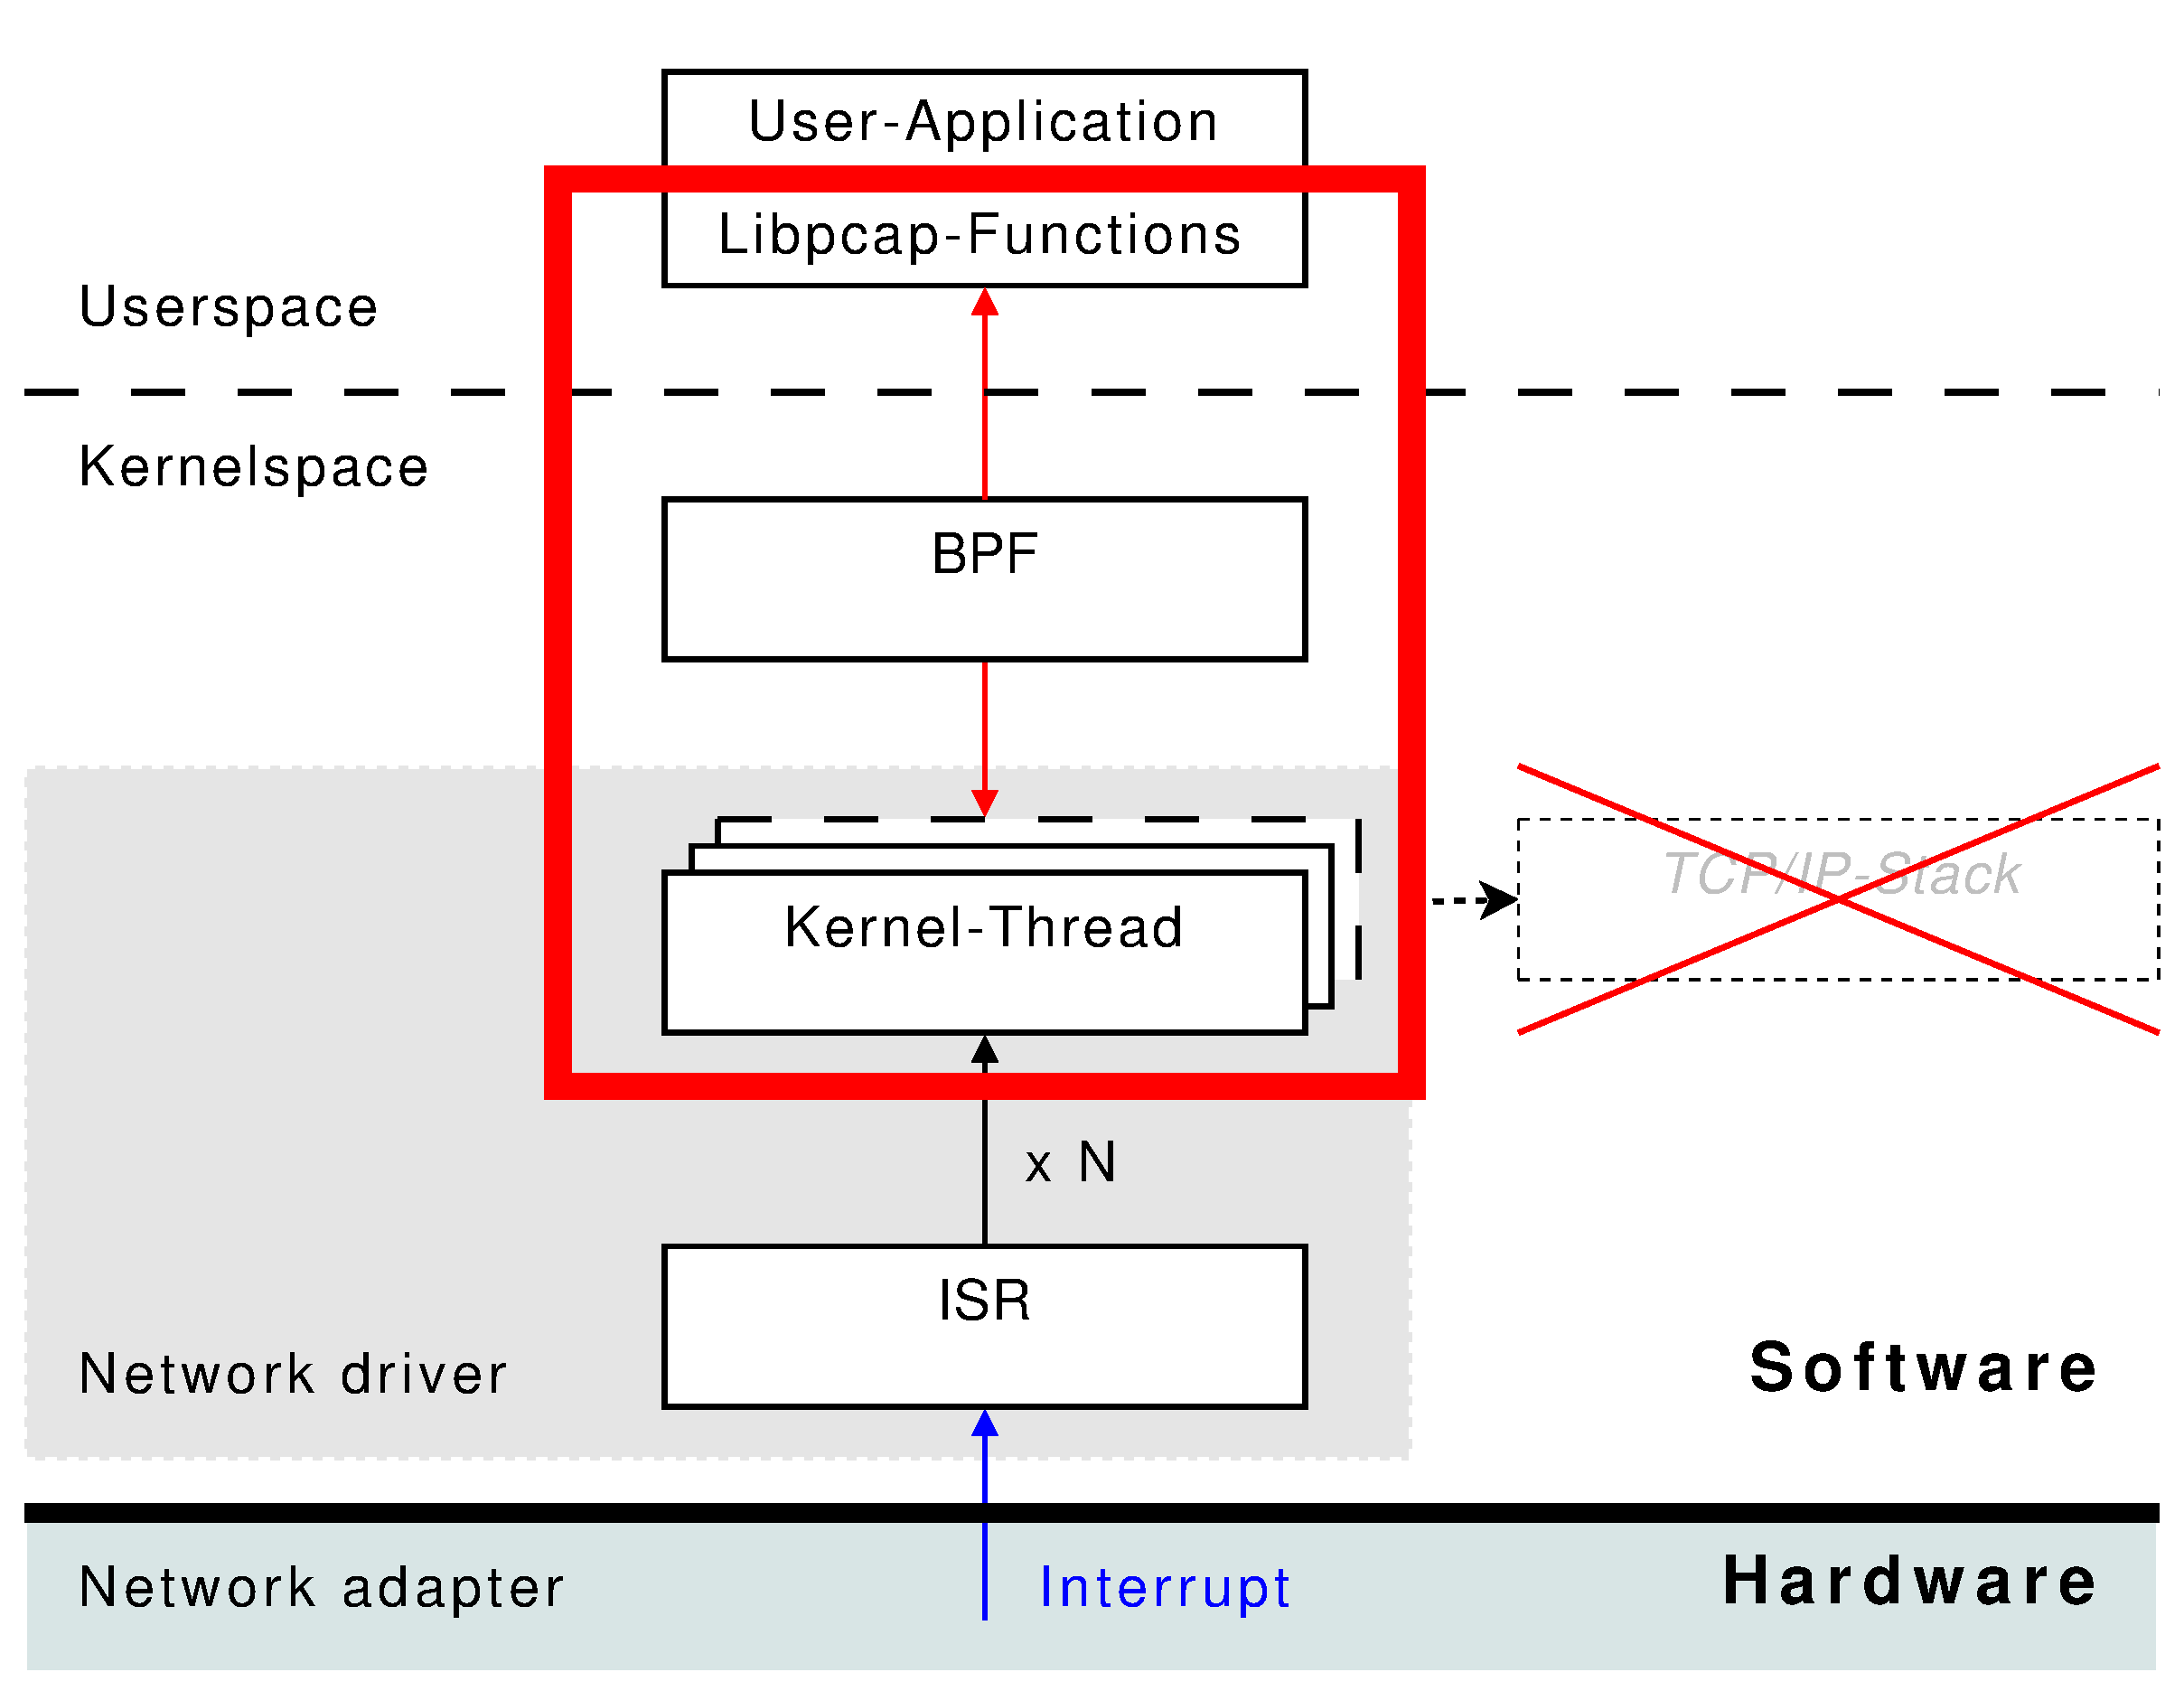
\includegraphics [height=55mm,width=60mm]{pics/PCS_funcs_ziel_DA}}
\end{columns}
\end{frame}

